\documentclass[tikz,border=10pt]{standalone}

\usepackage{amsmath}
\usetikzlibrary{matrix,positioning}

\begin{document}
  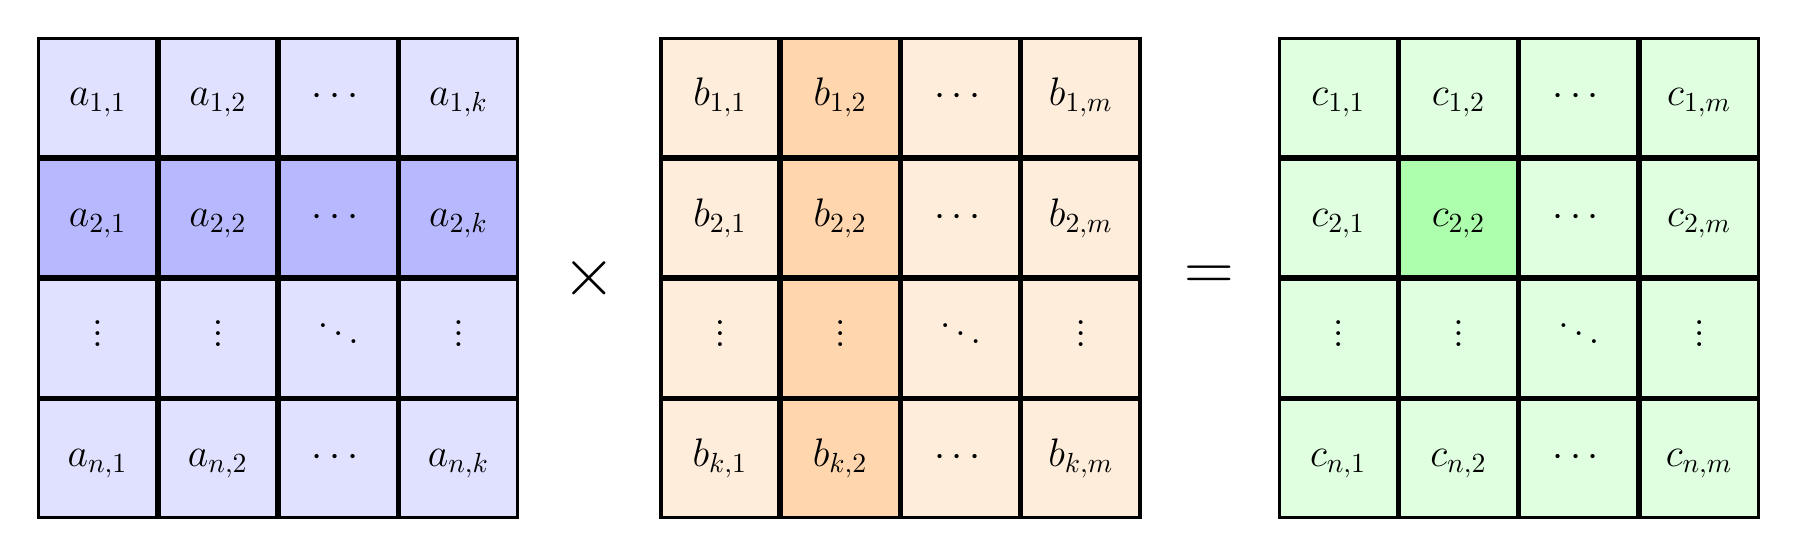
\begin{tikzpicture}[
    font=\Large,
    cell/.style={
      draw, very thick,
      minimum size=15mm,   % <- makes each cell quadratic (width = height)
      align=center
    },
    matA/.style={cell, fill=blue!12},
    matB/.style={cell, fill=orange!14},
    matC/.style={cell, fill=green!12},
    rowA/.style={cell, fill=blue!28},        % highlight full row in A
    colB/.style={cell, fill=orange!32},      % highlight full column in B
    hiC/.style={cell, fill=green!32},        % highlight single cell in C
    op/.style={font=\Huge},
    every matrix/.style={ampersand replacement=\&}
  ]

% A(4x4) * B(4x4) = C(4x4)
% Row 3 is dots in all matrices.
% Highlight: row 2 in A, column 2 in B, and only cell (2,2) in C.

% --- Matrix A (4x4), emphasize row 2 ---
    \matrix (A) [
      matrix of nodes,
      nodes in empty cells,
      nodes={text height=1.8ex, text depth=0.4ex},
      row sep=-\pgflinewidth,
      column sep=-\pgflinewidth
    ]{
      \node[matA] {$a_{1,1}$}; \& \node[matA] {$a_{1,2}$}; \& \node[matA] {$\cdots$}; \& \node[matA] {$a_{1,k}$}; \\
      \node[rowA] {$a_{2,1}$}; \& \node[rowA] {$a_{2,2}$}; \& \node[rowA] {$\cdots$}; \& \node[rowA] {$a_{2,k}$}; \\
      \node[matA] {$\vdots$};  \& \node[matA] {$\vdots$};  \& \node[matA] {$\ddots$}; \& \node[matA] {$\vdots$};  \\
      \node[matA] {$a_{n,1}$}; \& \node[matA] {$a_{n,2}$}; \& \node[matA] {$\cdots$}; \& \node[matA] {$a_{n,k}$}; \\
    };

% --- Multiplication sign ---
    \node[op, right=3mm of A] (times) {$\times$};

% --- Matrix B (4x4), emphasize column 2 ---
    \matrix (B) [
      matrix of nodes,
      nodes in empty cells,
      nodes={text height=1.8ex, text depth=0.4ex},
      row sep=-\pgflinewidth,
      column sep=-\pgflinewidth,
      right=3mm of times
    ]{
      \node[matB] {$b_{1,1}$}; \& \node[colB] {$b_{1,2}$}; \& \node[matB] {$\cdots$}; \& \node[matB] {$b_{1,m}$}; \\
      \node[matB] {$b_{2,1}$}; \& \node[colB] {$b_{2,2}$}; \& \node[matB] {$\cdots$}; \& \node[matB] {$b_{2,m}$}; \\
      \node[matB] {$\vdots$};  \& \node[colB] {$\vdots$};  \& \node[matB] {$\ddots$};  \& \node[matB] {$\vdots$};  \\
      \node[matB] {$b_{k,1}$}; \& \node[colB] {$b_{k,2}$}; \& \node[matB] {$\cdots$}; \& \node[matB] {$b_{k,m}$}; \\
    };

% --- Equals sign ---
    \node[op, right=3mm of B] (eq) {$=$};

% --- Matrix C (4x4), emphasize only cell (2,2) ---
    \matrix (C) [
      matrix of nodes,
      nodes in empty cells,
      nodes={text height=1.8ex, text depth=0.4ex},
      row sep=-\pgflinewidth,
      column sep=-\pgflinewidth,
      right=3mm of eq
    ]{
      \node[matC] {$c_{1,1}$}; \& \node[matC] {$c_{1,2}$}; \& \node[matC] {$\cdots$}; \& \node[matC] {$c_{1,m}$}; \\
      \node[matC] {$c_{2,1}$}; \& \node[hiC]  {$c_{2,2}$}; \& \node[matC] {$\cdots$}; \& \node[matC] {$c_{2,m}$}; \\
      \node[matC] {$\vdots$};  \& \node[matC] {$\vdots$};  \& \node[matC] {$\ddots$};  \& \node[matC] {$\vdots$};  \\
      \node[matC] {$c_{n,1}$}; \& \node[matC] {$c_{n,2}$}; \& \node[matC] {$\cdots$}; \& \node[matC] {$c_{n,m}$}; \\
    };

  \end{tikzpicture}
\end{document}